\documentclass{article}
\usepackage{import}
\subimport*{../}{macro}

\setlength\parindent{0px}

\begin{document}
\setcounter{aprob}{0}

{\centering
\Large\textbf{Homework \#1} \\[0.5em]
\normalsize CSEP 546: Machine Learning \\
Professor Jamie Morgenstern \\
Due: \textbf{Friday, April 24, 2026, 11:59pm} \\
57 points \\[1em]
}

\section*{A1 --- Short Answer and Conceptual Questions}

\subsubsection*{Solution:}

\begin{mdframed}
\textbf{\large Part a:} Bias, Variance, and the Bias-Variance Tradeoff
\end{mdframed}

\textbf{Bias} measures how far off a model's expected predictions are from the true values --- it's the systematic error that comes from wrong assumptions in the model, such as insufficient features, incorrect hyperparameters, or poor parameter selection.

Examples: (1) Fitting a straight line to data that's actually quadratic will consistently miss the curve no matter how much data you have. (2) A home sale price model that assigns high weight to exterior color or number of windows while missing key features like square footage --- it will systematically mis-estimate because the model's assumptions about what matters are wrong.

\medskip
\textbf{Variance} measures how much a model's predictions change when you train it on different samples of data. A high-variance model is overly sensitive to the specific training data it saw --- it picks up on noise and random fluctuations, deriving artificial patterns rather than learning the true underlying relationship.

Examples: (1) A model estimating a building's livable area that treats every roofline data point as meaningful signal --- minor measurement noise in the roofline causes wildly different area estimates across training sets. (2) A degree-20 polynomial fit to 15 data points --- it threads perfectly through the training data but produces completely different curves with a slightly different sample, because it's fitting noise rather than the true trend.

\medskip
\textbf{The bias-variance tradeoff:} Total prediction error decomposes as $\text{Error} = \text{Bias}^2 + \text{Variance} + \text{irreducible noise}$. Simple models (few parameters) tend to have high bias and low variance --- they underfit. Complex models (many parameters) tend to have low bias and high variance --- they overfit. Reducing one typically increases the other. The goal is to find the model complexity that minimizes total error --- flexible enough to capture the real pattern but constrained enough not to memorize noise.

The practical implication: it can be wise to use a biased estimator, so long as it reduces variance enough to lower the overall squared error (Murphy, chapter 6.4).

\bigskip
\begin{mdframed}
\textbf{\large Part b:} Effect of model complexity on bias and variance
\end{mdframed}

\textbf{When model complexity increases} (more parameters, higher degree polynomial, more features): bias typically decreases because the model has more flexibility to fit the true underlying pattern. But variance typically increases because the model becomes more sensitive to the specific training data, and each trading data point is inclusive of irreducible noise, variance on validation data will be higher.

\textbf{When model complexity decreases} (fewer parameters, stronger regularization, fewer features): bias typically increases because the model is too constrained to capture the true relationship. But variance typically decreases because the model is more stable across different training samples --- there's less room to overfit.

\textbf{Edge cases} When an included feature that has very minimal predictive weight (ex: house number/street name in the sale price estimation) complexity is increased, but may not really reflect on bias decreasing, and conversely removal of such feature/dimension may not increase variance since the model was depending on a noisy dimension to start with.

There are known techniques to control Variance like averaging over multiple models (ensembling), but bias cannot --- averaging equally biased models still produces a biased result.

\bigskip
\begin{mdframed}
\textbf{\large Part c:} Fewer features always generalize better?
\end{mdframed}

\boxed{\textbf{False.}}

Fewer features can improve generalization when the removed features are noisy or irrelevant, thus reducing variance and/or overfitting. But removing features that carry high predictive signal increases bias, and the model generalizes worse.

For example, predicting home prices using square footage + school rating generalizes well (both carry meaningful signal). Dropping school rating would hurt generalization because important predictive information is lost.

It depends on \textit{which} features are removed and whether the reduction in variance outweighs the increase in bias.

\bigskip
\begin{mdframed}
\textbf{\large Part d:} Hyperparameters should be tuned on the test set?
\end{mdframed}

\boxed{\textbf{False.}}

The test set exists to give an unbiased estimate of how the model will perform on unseen data. If hyperparameters are tuned on the test set, the model is effectively ``peeking'' at test data during training --- the test set is no longer unseen, and the produces (artificially) optimistic estimate for the model.

\bigskip
\begin{mdframed}
\textbf{\large Part e:} Training error overestimates true error?
\end{mdframed}

\boxed{\textbf{False.}}

Training error provides an \textbf{under}estimate of the true error. Since model's parameters were optimized specifically to minimize error on the training data, it will almost always perform better on the data it was trained on than on new, unseen data.

Example: complex models with a high-degree polynomial can achieve near-zero training error for every training point, while its true error on new data is would typically be much higher due to overfitting.

\noindent\rule{\textwidth}{0.4pt}

\clearpage{}
\section*{A2 --- Maximum Likelihood Estimation (MLE)}

\subsubsection*{Solution:}

\textbf{Known:}
\begin{itemize}
    \item Reign FC scored $[2, 4, 6, 0, 1]$ goals in 5 games. Model goals per game as Poisson with parameter $\lambda$
    \item Poisson distribution with parameter $\lambda$ probability of $\mathbb{Z}^+$ is
    \[
        \text{Poi}(x|\lambda) = e^{-\lambda} \frac{\lambda^x}{x!}
    \]
    \item log of the likelihood has the same maximizer as the likelihood function itself.
    \item $n$ games scores are iid.
\end{itemize}

\begin{mdframed}
\textbf{\large Part a:} Derive an expression for MLE
\end{mdframed}

Since $n$ game scores are iid, the joint probability is the product of individual probabilities:
\[
    L(\lambda) = \prod_{i=1}^{n} e^{-\lambda} \frac{\lambda^{x_i}}{x_i!}
\]

take the log of the likelihood - converts the product ($\prod$) into a sum ($\sum$):
\[
    \ell(\lambda) = \log L(\lambda) = \sum_{i=1}^{n} \left[ -\lambda + x_i \log \lambda - \log(x_i!) \right]
\]

rearrange pats of the sum with $x_i$ variable:
\[
    \ell(\lambda) = -n\lambda + \left(\sum_{i=1}^{n} x_i\right) \log \lambda - \sum_{i=1}^{n} \log(x_i!)
\]

Differentiate with respect to $d\lambda$:
\[
    \frac{d\ell}{d\lambda} = -n + \frac{\sum_{i=1}^{n} x_i}{\lambda}
\]

Set to zero and solve:
\[
    -n + \frac{\sum_{i=1}^{n} x_i}{\lambda} = 0
\]
\[
    \frac{\sum_{i=1}^{n} x_i}{\lambda} = n
\]
\[
    \hat{\lambda}_{\text{MLE}} = \frac{1}{n} \sum_{i=1}^{n} x_i = \bar{x}
\]

\textbf{Result:}

The MLE for $\lambda$ is the sample mean: $\boxed{\hat{\lambda} = \bar{x} = \frac{1}{n}\sum_{i=1}^{n} x_i}$

\bigskip
\begin{mdframed}
\textbf{\large Part b:} Numerical estimate of $P(6 \text{ goals})$ after 5 games score
\end{mdframed}

Calculate $\hat{\lambda}$:
\[
    \hat{\lambda} = \bar{x} = \frac{2+4+6+0+1}{5} = \frac{13}{5} = 2.60
\]

Probability of scoring exactly 6 goals next game $\Rightarrow P(X=6|\lambda=2.6)$:
\[
    P(X=6|\lambda=2.6) = e^{-2.6} \frac{2.6^6}{6!}
\]
\[
    \boxed{P(X=6|\lambda=2.6) \approx 0.03187}
\]

\bigskip
\begin{mdframed}
\textbf{\large Part c:} Numerical estimate of $P(6 \text{ goals})$ after 6 games score
\end{mdframed}

Calculate $\hat{\lambda}$:
\[
    \hat{\lambda} = \bar{x} = \frac{2+4+6+0+1+8}{6} = \frac{21}{6} = 3.50
\]

Probability of scoring exactly 6 goals next game $\Rightarrow P(X=6|\lambda=3.5)$:
\[
    P(X=6|\lambda=3.5) = e^{-3.5} \frac{3.5^6}{6!}
\]
\[
    \boxed{P(X=6|\lambda=2.6) \approx 0.06976}
\]

\noindent\rule{\textwidth}{0.4pt}

\clearpage{}
\section*{A3 --- Polynomial Regression}

\subsubsection*{Solution:}

\textbf{Observation of increasing regularization:} With $\lambda = 0$ and $d = 8$, the model overfits --- the curve threads through the training points, capturing irreducible noise rather than generalizing underlying pattern. Increasing $\lambda$ progressively constrains coefficient magnitudes, smoothing the curve and improving generalization up to a point ($\lambda \approx 0.1$), beyond which the model becomes too constrained and underfits --- losing the ability to capture the true relationship in the data.

\bigskip
\textbf{Plots} (all with $d = 8$):

\medskip
$\lambda = 0$ --- no regularization. The curve overfits, threading through training points and capturing noise.
\begin{center}
    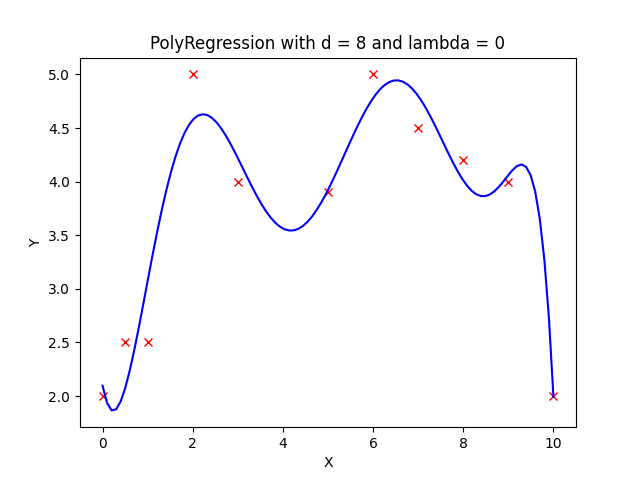
\includegraphics[width=4.5in]{./before_reg_d8_lambda0.png}
\end{center}

\medskip
$\lambda = 0.1$ --- the curve is smoother and appears to generalize well, maintaining close fit to the data points with minimal squared error.
\begin{center}
    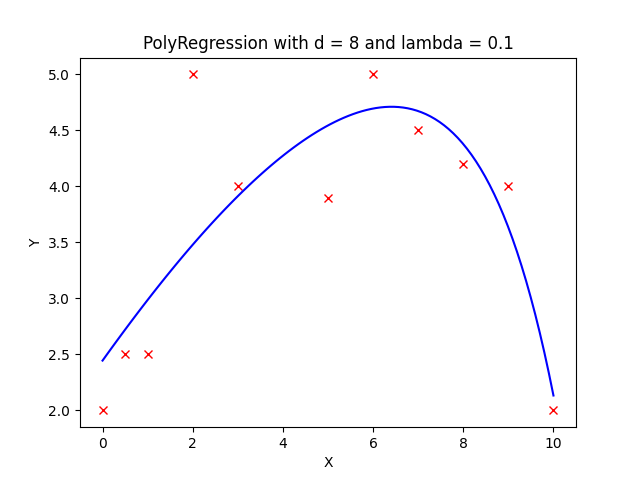
\includegraphics[width=4.5in]{./after_reg_d8_lambda0.1.png}
\end{center}

\medskip
$\lambda = 0.5$ --- the curve begins to underfit; data points near the origin start falling outside the fitted pattern.
\begin{center}
    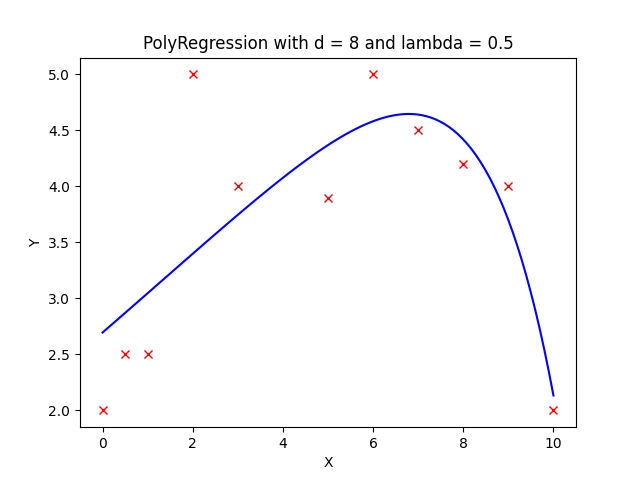
\includegraphics[width=4.5in]{./after_reg_d8_lambda0.5.png}
\end{center}

\medskip
$\lambda = 1.0$ --- the lower half of the curve becomes nearly linear, missing the structure of data points near the origin.
\begin{center}
    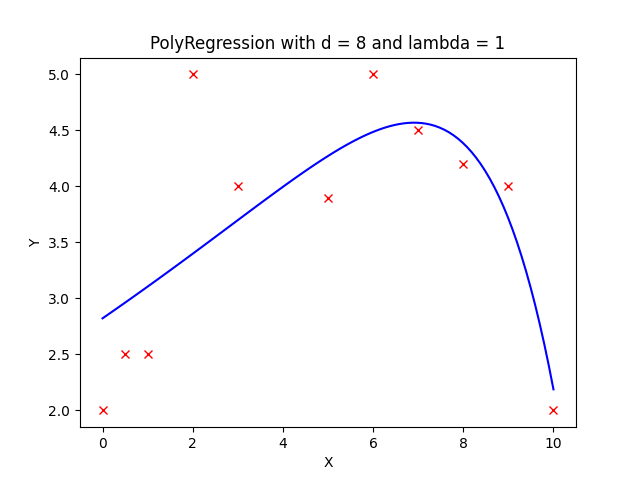
\includegraphics[width=4.5in]{./after_reg_d8_lambda1.png}
\end{center}

\medskip
$\lambda = 5.0$ --- the curve is largely flattened, only fitting the central tendency of the data and missing most of the underlying pattern.
\begin{center}
    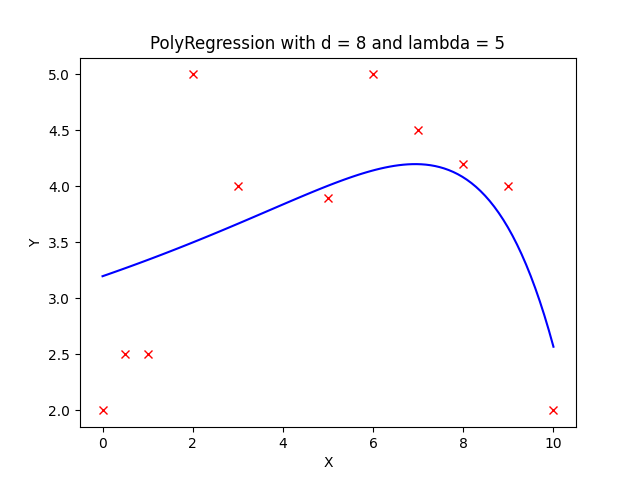
\includegraphics[width=4.5in]{./after_reg_d8_lambda5.png}
\end{center}

\noindent\rule{\textwidth}{0.4pt}

\clearpage{}
\section*{A4 --- Polynomial Regression: Learning Curves}

\subsubsection*{Solution:}

\textbf{Observations from Required plots} for $(d, \lambda) \in \{(1,0), (4,10^{-6}), (8,10^{-6}), (8,0.1), (8,1), (8,100)\}$

\begin{center}
    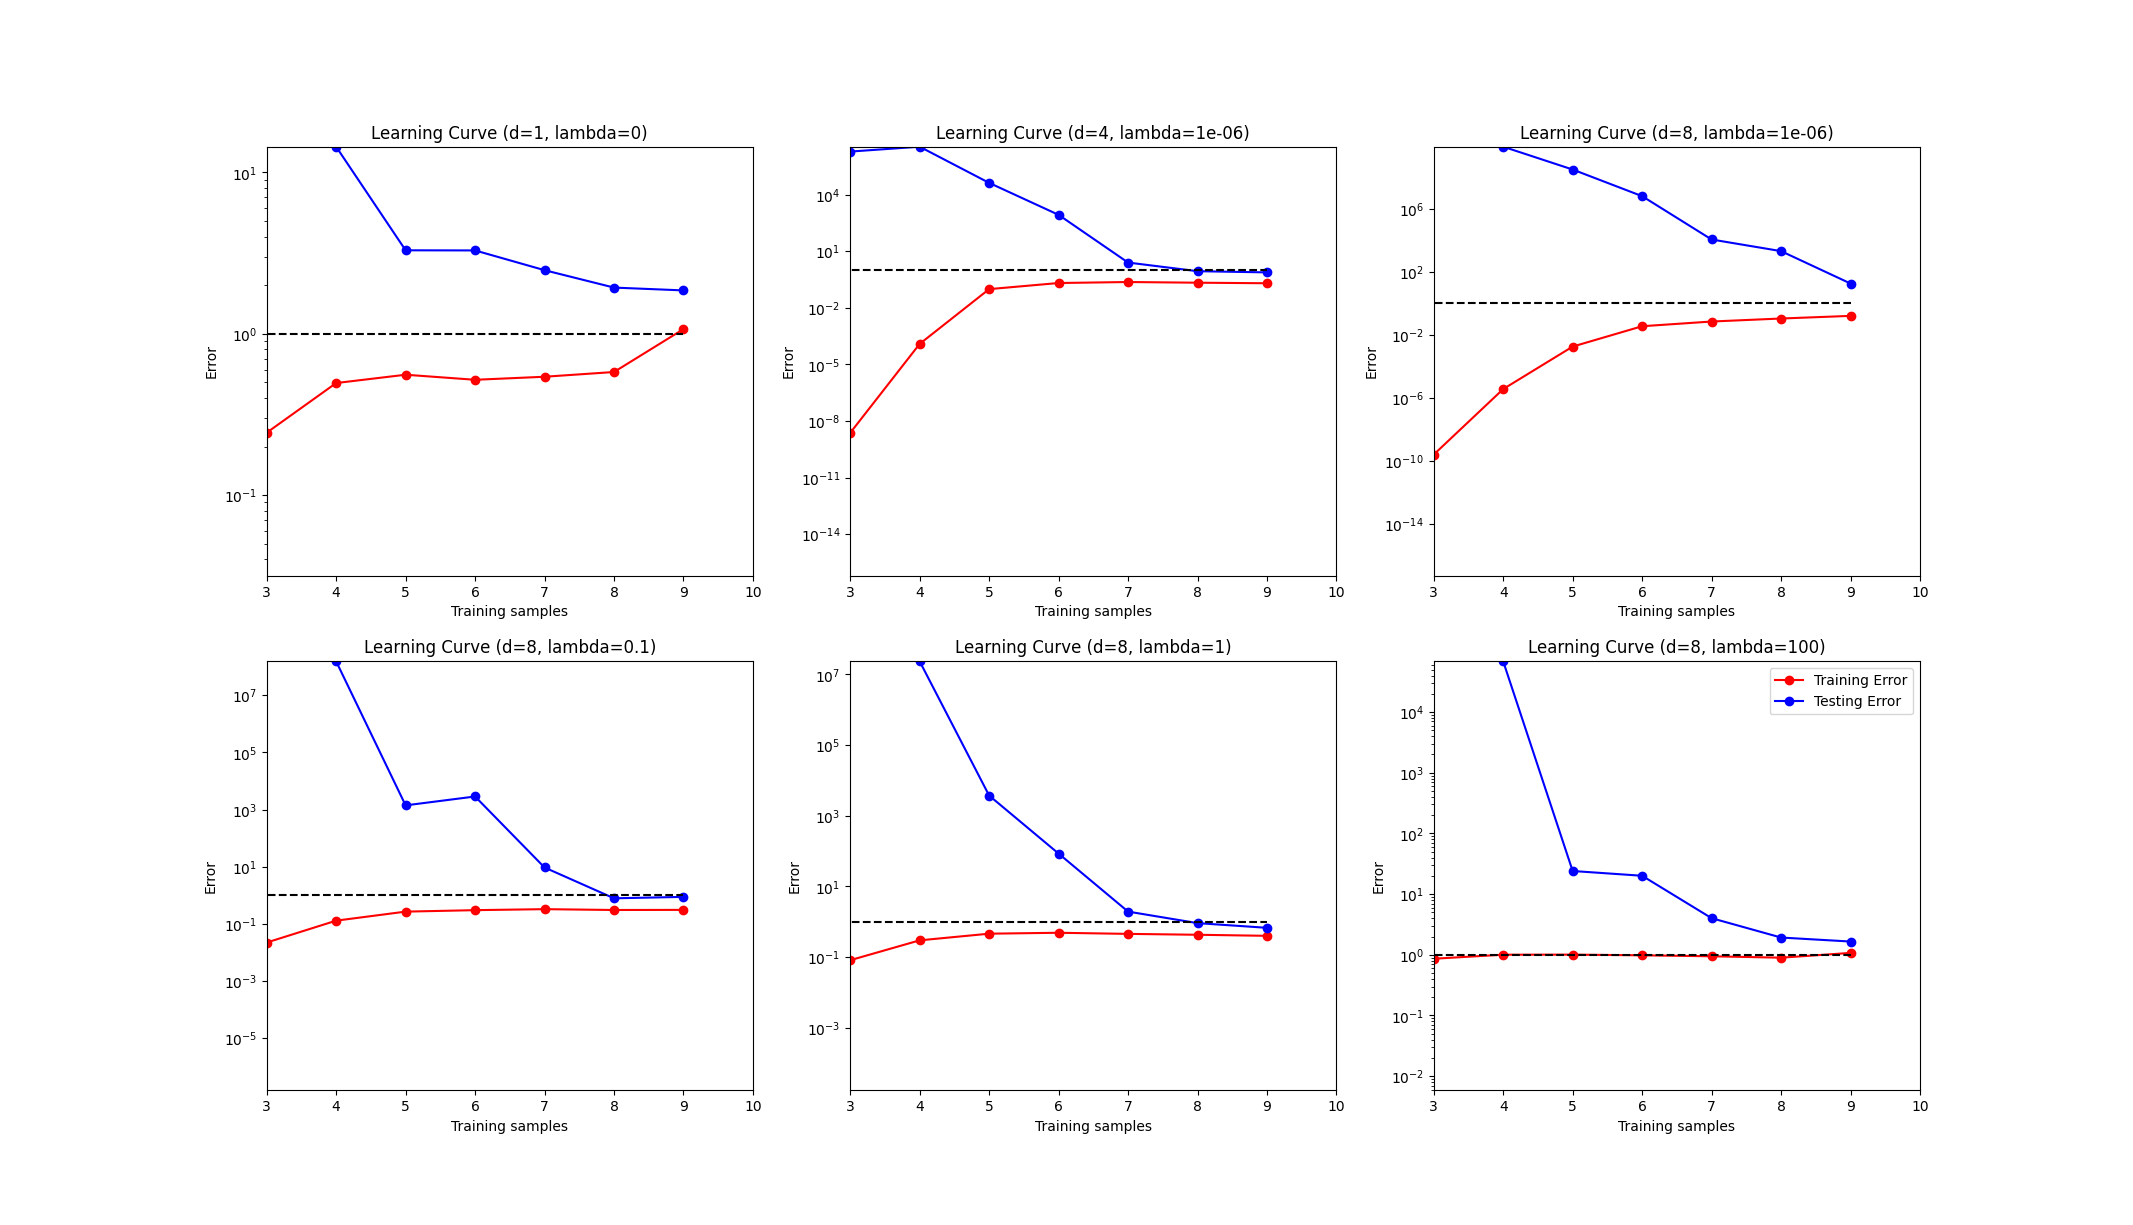
\includegraphics[width=\textwidth]{./learning_curves.png}
\end{center}

Increasing $d$ from 1$\rightarrow$4$\rightarrow$8 with minimal regularization shows bias decreasing (training error drops) but variance increasing (train-test gap widens dramatically). At d=8, $\lambda$=1e-6, test error reaches $10^6$ --- severe overfitting.

Increasing $\lambda$ from 1e-6$\rightarrow$0.1$\rightarrow$1$\rightarrow$100 at fixed d=8 shows the reverse: the train-test gap narrows (variance decreasing) while both errors gradually rise (bias increasing). At $\lambda$=1, training and test error converge near the dashed line --- the best tradeoff. At $\lambda$=100, both errors are high --- effectively underfitting, similar to d=1.

\bigskip
\textbf{Observations from Additional exploratory plots} for $(d, \lambda) \in \{(2,10^{-6}), (4,0.1), (6,0.1), (8,0.01), (8,0.5), (8,10)\}$

\begin{center}
    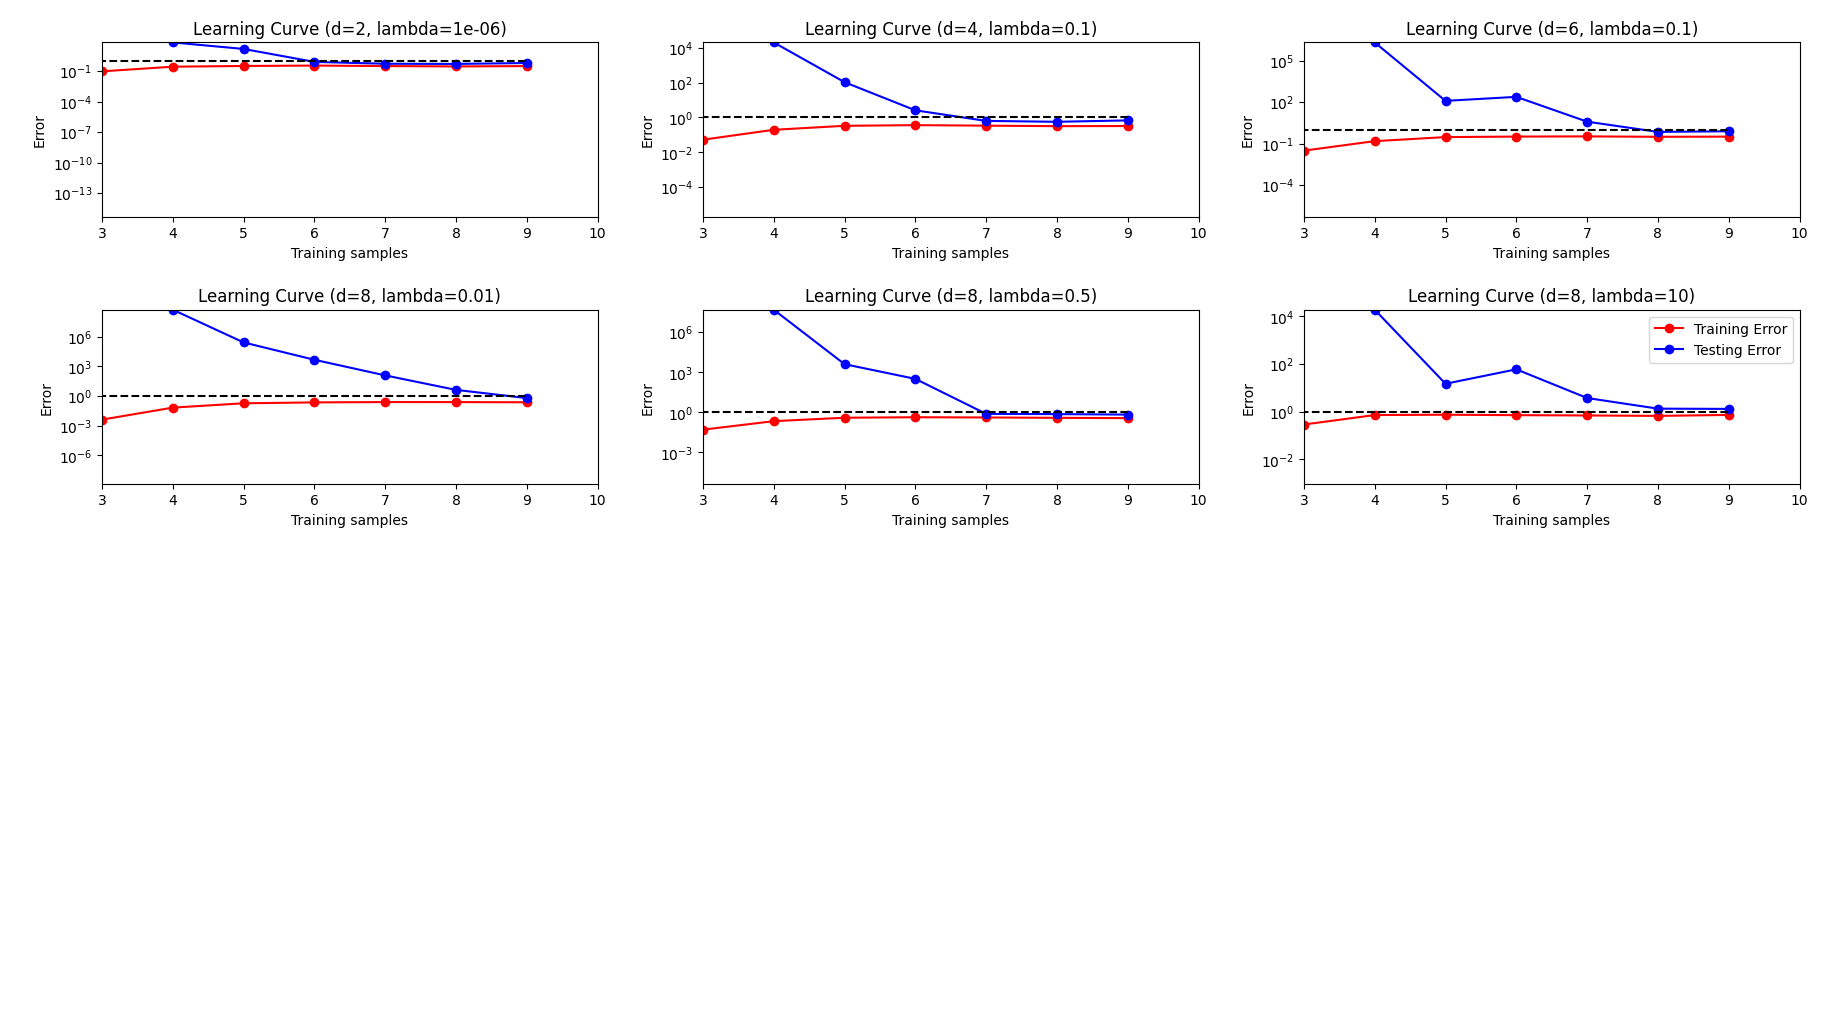
\includegraphics[width=\textwidth]{./exploratory_plots.png}
\end{center}

Multiple $(d, \lambda)$ combinations achieve similar performance --- $(d=4, \lambda=0.1)$, $(d=6, \lambda=0.1)$, and $(d=8, \lambda=0.5)$ all show tight convergence of training and test error. This confirms there is no single ``correct'' model --- rather a family of solutions that balance bias and variance differently.

The sweet spot for d=8 lies around $\lambda \in [0.5, 1]$, with $\lambda$=0.01 still overfitting and $\lambda$=10 already underfitting.

\noindent\rule{\textwidth}{0.4pt}

\clearpage{}
\section*{A5 --- Ridge Regression on MNIST}

\textbf{Known:}
\begin{itemize}
    \item MNIST dataset: 28$\times$28 grayscale images of digits 0-9, flattened to $x_i \in \R^d$ where $d = 784$
    \item Labels $z_j \in \{0, \ldots, 9\}$, one-hot encoded as $y_i \in \{0,1\}^k$ where $k = 10$
    \item One-hot encoding: label $z$ maps to $e_{z+1}$ (standard basis vector with 1 at position $z+1$)
    \item Weight matrix $W \in \R^{d \times k}$, with columns $W = [w_1 \ldots w_k]$
    \item Frobenius norm: $\|W\|_F^2 = \sum_{i=1}^{d} \sum_{j=1}^{k} W_{i,j}^2$
    \item $X = [x_1 \ldots x_n]^\top \in \R^{n \times d}$ (data matrix, each row is one image)
    \item $Y = [y_1 \ldots y_n]^\top \in \R^{n \times k}$ (label matrix, each row is one-hot vector)
\end{itemize}

\subsubsection*{Solution:}

\begin{mdframed}
\textbf{\large Part a:} Derive the closed-form expression for $\hat{W}$
\end{mdframed}

Objective: minimize the regularized least squares
\[
    \hat{W} = \text{argmin}_{W \in \R^{d \times k}} \sum_{i=1}^{n} \|W^T x_i - y_i\|_2^2 + \lambda\|W\|_F^2
\]

\medskip
\textbf{Step 1: Decompose the Frobenius norm by columns}

Since $W = [w_1 \ldots w_k]$, the Frobenius norm decomposes as:
\[
    \|W\|_F^2 = \sum_{j=1}^{k} \|w_j\|_2^2
\]
each column's squared norm contributes independently to the total penalty.

\medskip
\textbf{Step 2: Decompose the data error term by columns}

$W^T x_i$ is a $k$-dimensional vector. Its $j$-th entry is $e_j^T W^T x_i = w_j^T x_i$

$y_i$'s $j$-th entry is $e_j^T y_i$

So the squared error for one data point decomposes:
\[
    \|W^T x_i - y_i\|_2^2 = \sum_{j=1}^{k} (w_j^T x_i - e_j^T y_i)^2
\]

\medskip
\textbf{Step 3: Combine and rearrange the full objective}

Substituting the decompositions into the objective:
\[
    \sum_{i=1}^{n} \|W^T x_i - y_i\|_2^2 + \lambda\|W\|_F^2 = \sum_{j=1}^{k} \left[ \sum_{i=1}^{n} (w_j^T x_i - e_j^T y_i)^2 + \lambda\|w_j\|_2^2 \right]
\]

The inner sum over $i$ can be written in matrix form. Since $w_j^T x_i$ is the $i$-th entry of $Xw_j$, and $e_j^T y_i$ is the $i$-th entry of $Ye_j$ (the $j$-th column of $Y$):
\[
    = \sum_{j=1}^{k} \left[ \|Xw_j - Ye_j\|_2^2 + \lambda\|w_j\|_2^2 \right]
\]

\medskip
\textbf{Step 4: Each column is an independent ridge regression}

The objective is a sum over $j = 1, \ldots, k$ where each term only involves $w_j$. Minimizing the total = minimizing each term independently.

For each $j$, the problem is:
\[
    \hat{w}_j = \text{argmin}_{w_j} \|Xw_j - Ye_j\|_2^2 + \lambda\|w_j\|_2^2
\]
This is standard ridge regression with target vector $Ye_j$ (the $j$-th column of $Y$).

\medskip
\textbf{Step 5: Solve each ridge regression}

Expand the objective for column $j$:
\[
    \|Xw_j - Ye_j\|_2^2 + \lambda\|w_j\|_2^2 = (Xw_j - Ye_j)^T(Xw_j - Ye_j) + \lambda w_j^T w_j
\]
\[
    = w_j^T X^T X w_j - 2w_j^T X^T Y e_j + e_j^T Y^T Y e_j + \lambda w_j^T w_j
\]

Differentiate with respect to $w_j$ and set to zero:
\[
    \frac{\partial}{\partial w_j} = 2X^T X w_j - 2X^T Y e_j + 2\lambda w_j = 0
\]
\[
    (X^T X + \lambda I) w_j = X^T Y e_j
\]
\[
    \hat{w}_j = (X^T X + \lambda I)^{-1} X^T Y e_j
\]

\medskip
\textbf{Step 6: Stack all columns back into W}

Since $\hat{w}_j = (X^T X + \lambda I)^{-1} X^T Y e_j$ for each $j = 1, \ldots, k$

And $[Ye_1 \; Ye_2 \; \ldots \; Ye_k] = Y$ (selecting each column of $Y$ reconstructs $Y$)

Stacking all columns: $\hat{W} = [\hat{w}_1 \ldots \hat{w}_k] = (X^T X + \lambda I)^{-1} X^T [Ye_1 \ldots Ye_k]$
\[
    \boxed{\hat{W} = (X^T X + \lambda I)^{-1} X^T Y}
\]

\textbf{Result:}
\[
    \hat{W} = (X^T X + \lambda I)^{-1} X^T Y
\]

The multi-class ridge regression decomposes into $k$ independent single-output regression per class. Each shares the $(X^T X + \lambda I)^{-1} X^T$ factor --- only target column of $Y$ differs.

\bigskip
\begin{mdframed}
\textbf{\large Part b:} Implementation
\end{mdframed}

\textbf{Results} with $\lambda = 10^{-4}$:
\begin{itemize}
    \item Training error: $\boxed{14.805\%}$
    \item Testing error: $\boxed{14.66\%}$
\end{itemize}

\medskip
\textbf{\texttt{one\_hot(y, num\_classes)}} --- converts integer label vector to binary matrix
\begin{itemize}
    \item Input: $y \in \{0, \ldots, k-1\}^n$ (integer labels), $k$ = number of classes
    \item Output: $Y \in \{0,1\}^{n \times k}$ where each row has a single 1 at the column matching the label
    \item Example: $y = [2, 3, 1, 0]$ with $k=4$ produces rows $[0,0,1,0], [0,0,0,1], [0,1,0,0], [1,0,0,0]$
    \item Use NumPy fancy indexing: create an $n \times k$ zeros matrix, then set \texttt{result[i, y[i]] = 1} for all $i$ simultaneously
\end{itemize}

\medskip
\textbf{\texttt{train(X, Y, $\lambda$)}} --- computes $\hat{W} = (X^T X + \lambda I)^{-1} X^T Y$
\begin{itemize}
    \item Compute $A = X^T X + \lambda I$ where $I$ is the $d \times d$ identity matrix
    \item Compute $B = X^T Y$
    \item Solve $AW = B$ for $W$ using \texttt{np.linalg.solve(A, B)} --- do NOT explicitly compute $A^{-1}$
    \item Why \texttt{solve} instead of inverse: solving the linear system directly is faster and more numerically stable. The problem hint states ``if you are inverting a matrix, you are probably doing something wrong.''
\end{itemize}

\medskip
\textbf{\texttt{predict(X, W)}} --- classifies new inputs
\begin{itemize}
    \item Compute scores: $S = XW$ where $S \in \R^{n \times k}$ --- each row is a score vector over $k$ classes
    \item For each row, pick the class with the highest score: $\hat{z}_i = \text{argmax}_j \; S_{i,j}$
    \item Returns integer predictions $\in \{0, \ldots, 9\}$
\end{itemize}

\end{document}
